%!TEX root =./main.tex
% arara: pdflatex
% arara: makeglossaries
% arara: biber 
% arara: pdflatex while changed('bbl') || changed('gls') || found('log', 'Please rerun') || found('log', 'Label(s) may have changed')

%%**************************************************************
%%
%% DHBW Heidenheim - Template for Bachelor Thesis
%%
%% Bevor usisng this template please have a look at the REAMDME.md file
%%
%%**************************************************************

%!TEX root =../main.tex

% show warning for old LaTeX syntax
\RequirePackage[l2tabu, orthodox]{nag}

\documentclass[
    pdftex,
    oneside,
    12pt,			        % fontsize
    parskip=half,		    % Space (in lines) between paragraphs
    headheight = 20pt,      % Header hight
    headsepline,		    % Line after header
    footheight = 16pt,	    % Footer height
    footsepline,		    % Line before footer
    abstract=true,		    % Abstract headline
    DIV=calc,		        % Calculate print space
    BCOR=8mm,		        % BCOR settings (Bindekorrektur)
    headinclude=false,      % Exclude header from print space
    footinclude=false,	    % Exclude footer from print space
    listof=totoc,		    % Show List of Figures/Tables in Contents
    toc=bibliography,	    % Show Bibliography in Contents
    % appendixprefix = true
]{scrreprt}	                % Koma-Script report-class, long document: scrreprt, short document: scrbook

\usepackage{xstring}
\usepackage[utf8]{inputenc}
\usepackage[T1]{fontenc}

\usepackage{xcolor}

\usepackage{pifont}

% iflang command definition
\newcommand{\iflang}[2]{%
    \IfStrEq{\documentLanguage}{#1}{#2}{}%
}

% ifDocType comand definition
\newcommand{\ifDocType}[3]{%
    \IfStrEq{\documentType}{#1}{#2}{#3}%
}

% ifMultipleAuthors definition
\newcommand{\ifMultipleAuthors}[2]{%
    \IfStrEq{\multipleAuthors}{true}{#1}{#2}%
}

% ifSpecialDocument definition
\newcommand{\ifSpecialDocument}[2]{\IfStrEqCase{\documentType}{%
        {T2_1000}{#2\ignorespaces}%
            {T2000}{#2\ignorespaces}%
            {T3100}{#2\ignorespaces}%
            {T3300}{#2\ignorespaces}%
    }[#1\ignorespaces]%
}


% Include main settings
%!TEX root = ../main.tex

%% Citation Styles
% https://de.overleaf.com/learn/latex/Biblatex_citation_styles
% recommended: for Electrical Engineering/Computer Science: IEEE
% DHBW Heilbronn Guideline says: authoryear (Harvard-Style)
\newcommand{\quoteStyle}{ieee}

%% Fonts
%% palatino, goudysans, lmodern or libertine
\newcommand{\documentFont}{lmodern}

%% Margin
\newcommand{\margin}{2.5cm}

%% Space between chapter headline and top of page
\newcommand{\chapterMargin}{20pt}

%% Table settings
% Column spacing
\newcommand{\tableColumnMargin}{10pt}
%Line spacing
\newcommand{\tableRowMargin}{1.5}

%% Color settings
\newcommand{\defineColors}{%
	\definecolor{LinkColor}{HTML}{\linkColor}
	\definecolor{ListingBackground}{HTML}{F8F8F8}
}

%% Syntax Highlighting (Listings)
\newcommand{\listingsettings}{%
	\lstset{%
		language=Java,				% default language
		numbers=left,				% position of line numbers (left, right)
		stepnumber=1,				% set number to each line
		numbersep=5pt,				% 5pt between number and source code
		numberstyle=\tiny,			% letter size of numbers
		breaklines=true,		    % break lines if necessary (true, false)
		breakautoindent=true,	    % indenting after break line (true, false)
		postbreak=\space,			% break line after space
		tabsize=2,					% tabulator size
		basicstyle=\ttfamily\footnotesize, % font style
		showspaces=false,			% show space (true, false)		showstringspaces=false,		% show space in strings (true, false)
		extendedchars=true,			% show all Latin1 characters (true, false)
		captionpos=b,				% sets the caption-position to bottom
		backgroundcolor=\color{ListingBackground}, % source code background
		xleftmargin=10pt,		    % margin left
		xrightmargin=5pt,		    % margin right
		frame=single,			    % border settings
		frameround=ffff,
		rulecolor=\color{darkgray},	% border color
		fillcolor=\color{ListingBackground},
		aboveskip=20pt,
		keywordstyle=\color[rgb]{0.133,0.133,0.6},
		commentstyle=\color[rgb]{0.133,0.545,0.133},
		stringstyle=\color[rgb]{0.627,0.126,0.941}
	}
}


% Include document settings
%!TEX root = ../main.tex

%% Document language (en, de)
\newcommand{\documentLanguage}{de}

%% Document type
% T1000 Project Thesis (Semester 1 & 2)
% T2000 Project Thesis (Semester 3 & 4)
% T3100 Seminar Paper (Semester 5 & 6)
% T3300 Bachelor Thesis
% or custom type like 'Hausarbeit'
\newcommand{\documentType}{T2000}
\newcommand{\showCompanyLogo}{true}

\newcommand{\multipleAuthors}{false}
\newcommand{\documentAuthor}{Max Mustermensch}
\newcommand{\documentTitle}{Titel der Arbeit}
\newcommand{\documentPeriod}{12 Wochen}

\newcommand{\matriculationNumber}{1234510}
\newcommand{\dateOfBirth}{01.01.1999}
\newcommand{\placeOfBirth}{Geburtsort}


\newcommand{\locationUniversity}{Heilbronn}
\newcommand{\department}{Wirtschaftsinformatik}
\newcommand{\course}{WI23A3}

\newcommand{\degree}{Bachelor of Science}
% INF2014 - INF2016 (MI):       Bachelor of Science
% INF2014 - INF2016 (IA/IM) :   Bachelor of Engineering
% INF2017 (all):                Bachelor of Science

% A lecture that the document is written for
\newcommand{\lecture}{Software Engineering}
% Whether to show the lecture on cover
\newcommand{\showLecture}{false}

\newcommand{\releaseDate}{September 2077}
\newcommand{\releaseLocation}{Heilbronn}

\newcommand{\companyName}{Firma GmbH}
\newcommand{\companyLocation}{Firmenort}

\newcommand{\tutor}{Dipl.-Ing.~(FH) Peter Pan}
\newcommand{\evaluator}{Prof. Dr.\ Albert Einstein}

\newcommand{\linkColor}{000000}


% Load language specific Strings
\input{lang/\documentLanguage}

% Load language specific babel package
\iflang{de}{\usepackage[english, ngerman]{babel}}
\iflang{en}{\usepackage[ngerman, english]{babel}}

% Add comment feature
\newcommand{\comment}[1]{\par {\bfseries \color{blue} #1 \par}}


%%%%%%% Package Includes %%%%%%%
\usepackage[margin=\margin, foot=1cm]{geometry}
\usepackage[onehalfspacing]{setspace}
\usepackage{makeidx}
\usepackage[autostyle=true,german=quotes]{csquotes}
\usepackage{enumitem}
\usepackage{graphicx}
\usepackage{pdfpages}
\usepackage{float}
\usepackage{calc}
\usepackage{wrapfig}
\usepackage[perpage, hang, multiple, stable, bottom]{footmisc}
\usepackage{listings}
\usepackage{amsmath}
\usepackage{amssymb}
\usepackage{\documentFont}
\usepackage[%
    pdftitle={\documentTitle},
    pdfauthor={\documentAuthor},
    pdfsubject={\documentType},
    pdfcreator={pdflatex, LaTeX with KOMA-Script},
    pdfpagemode=UseOutlines,        % Show Contents while opening
    pdfdisplaydoctitle=true, 		% Show document title instead of file name
    pdflang={\documentLanguage},    % Document language
]{hyperref}
\usepackage{bookmark}
\usepackage[nonumberlist,toc,acronym,nopostdot]{glossaries}
\usepackage{scrhack}
\usepackage{tabularx}
\usepackage{afterpage}

% Appendix
\usepackage[toc, page, title, titletoc, header]{appendix}
\renewcommand{\appendixname}{\appendixPhrase}
\renewcommand{\appendixtocname}{\appendixPhrase}
\renewcommand{\appendixpagename}{\appendixPhrase}
\renewcommand{\autodot}{}

% Seperate Appendix TOC
\DeclareNewTOC[%
    owner=\jobname,
    listname={\appendixtocPhrase},% title of the appendix ToC
]{atoc}

\makeatletter
\newcommand*\appendixtoc{%
    \renewcommand*{\ext@toc}{atoc}%
    \scr@ifundefinedorrelax{hypersetup}{}{\hypersetup{bookmarkstype=atoc}}%
    \listofatocs
}
\makeatother

% Generate glossary
\makeglossaries{}

% Load colors
\defineColors{}

% Set Titel, Autor and Date
\title{\documentTitle}
\author{\documentAuthor}
\date{\datum}


% PDF link settings
\hypersetup{%
    colorlinks=true,
    linkcolor=LinkColor,
    citecolor=LinkColor,
    filecolor=LinkColor,
    menucolor=LinkColor,
    urlcolor=LinkColor,
    linktocpage=true,
    bookmarksnumbered=true
}

% Captions fontsize
\addtokomafont{caption}{\small}

% Bibliographie settings
\iflang{de}{%
    \usepackage[
        backend=biber,		 % recommended. Alternative: bibtex
        bibwarn=true,
        bibencoding=utf8,	 % If.bib file is encoded with utf8, otherwise ascii
        sortlocale=de_DE,
        style=\quoteStyle,
        maxnames=5,
        minnames=4,
        dashed=false
    ]{biblatex}
    \DefineBibliographyStrings{german}{andothers={et\addabbrvspace al\adddot}}
}
\iflang{en}{%
    \usepackage[
        backend=biber,		 % recommended. Alternative: bibtex
        bibwarn=true,
        bibencoding=utf8,    % If.bib file is encoded with utf8, otherwise ascii
        sortlocale=en_US,
        style=\quoteStyle,
        maxnames=5,
        minnames=4,
        dashed=false
    ]{biblatex}
}

\setcounter{biburllcpenalty}{7000}
\setcounter{biburlucpenalty}{8000}

% \bibliography{bibliographie.bib}
\addbibresource{bibliographie.bib}

% Hurenkinder und Schusterjungen verhindern
% http://projekte.dante.de/DanteFAQ/Silbentrennung
\clubpenalty = 10000 % schließt Schusterjungen aus (Seitenumbruch nach der ersten Zeile eines neuen Absatzes)
\widowpenalty = 10000 % schließt Hurenkinder aus (die letzte Zeile eines Absatzes steht auf einer neuen Seite)
\displaywidowpenalty=10000

% Graphicspath
\graphicspath{{images/}}

% frequently used programing languages
\lstloadlanguages{PHP,Python,Java,C,C++,bash}

\listingsettings{}
% Rename Listings
\renewcommand\lstlistingname{\listingPhrase}
\renewcommand\lstlistlistingname{\listListingPhrase}
\def\lstlistingautorefname{\authorListingPhrase}

% Spaces in tables
\setlength{\tabcolsep}{\tableColumnMargin}
\renewcommand{\arraystretch}{\tableRowMargin}


%!TEX root = ../main.tex

%
% To create glossary run the following command: 
% makeglossaries main.acn && makeglossaries main.glo
%

%
% Glossareintraege --> referenz, name, beschreibung
% Aufruf mit \gls{...}

\newglossaryentry{Glossareintrag}{name={Glossareintrag},plural={Glossareinträge},description={Ein Glossar beschreibt verschiedenste Dinge in kurzen Worten}}

% Abkürzungen

\newacronym{AGPL}{AGPL}{Affero GNU General Public License}


\begin{document}

% Cover
\begin{spacing}{1}
    %!TEX root = ../main.tex

\begin{titlepage}

    
\includegraphics[height=2.5cm]{images/cover/logo-dhbw.pdf}
    \IfStrEq{\showCompanyLogo}{true}{
        \hfill
        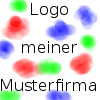
\includegraphics[height=2.5cm]{images/cover/logo-company.png}
    }
    
    \enlargethispage{20mm}
    \begin{center}
        \doublespacing{
            \vspace*{12mm}
            {\LARGE\textbf\documentTitle}
        }\\
        \vspace*{12mm}
        {\large\textbf\documentTypePhrase}\\

        % degree only for bachelor thesis
        \ifDocType{T3300}{
            \vspace*{12mm}
            \degreePhrase\\
            \vspace*{3mm}
            {\textbf\degree}\\
        }

        \IfStrEq{\showLecture}{true}{
            \vspace*{12mm}
            \lecturePhrase\\
            \vspace*{0mm}
            {\textbf\lecture}\\
        }

        \vspace*{12mm}\departmentPhrase\ \department\\
        \vspace*{0mm}\locationUniversityPhrase\ \locationUniversity\\
        \vspace*{12mm}\documentAuthorPhrase\\
        \vspace*{3mm}
        {\large\textbf\documentAuthor}\\
        \vspace*{12mm}\releaseDate\\
        \vfill
        \begin{spacing}{0.8}
            \begin{tabularx}{\textwidth}{XX}
                \textbf{\documentPeriodPhrase}                     & \documentPeriod                \\
                \textbf{\matriculationNumberPhrase, \coursePhrase} & \matriculationNumber, \course  \\
                \textbf{\dateOfBirthPhrase, \placeOfBirthPhrase}   & \dateOfBirth, \placeOfBirth    \\
                \textbf{\companyPhrase}                            & \companyName, \companyLocation \\
                \textbf{\tutorPhrase}                              & \tutor                         \\
                \textbf{\evaluatorPhrase}                          & \evaluator
            \end{tabularx}
        \end{spacing}
    \end{center}
\end{titlepage}

\end{spacing}
\newpage

\pagenumbering{Roman}

% Restriction notices
\ifDocType{T3100}{%
    % no restricition notices for semester paper
}{%
    %!TEX root = ../main.tex

\thispagestyle{empty}

\section*{\restrictionNoticesPhrase}

\vspace*{2em}

\iflang{de}{%
  Die vorliegende Arbeit beinhaltet vertrauliche Informationen der Firma {\companyName}.
  Sie ist nur für die Beteiligten am Begutachtungs- und Evaluationsprozess bestimmt.

  Die Weitergabe des Inhalts der Arbeit im Ganzen oder von Teilen daraus an externe Dritte sowie das Anfertigen von Abschriften oder Kopien zu welchem Zweck, in welcher Form und zu welchem Zeitpunkt auch immer, sind grundsätzlich untersagt.

  Ausnahmen bedürfen der schriftlichen Genehmigung der Firma {\companyName}.
  Eine Weitergabe an Mitarbeiter der Hochschule aufgrund fachlicher Belange oder für administrative Zwecke ist von dieser Regelung explizit ausgenommen.
}

%http://www.ib.dhbw-mannheim.de/fileadmin/ms/bwl-ib/Downloads_alt/Leitfaden_31.05.pdf

\iflang{en}{%
  The {\documentTypePhrase} on hand
  \begin{center}{\itshape{} \documentTitle{}\/}\end{center}
  contains internal resp.\ confidential data of {\companyName}. It is intended solely for inspection by the
  assigned examiner, the head of the {\department} department and, if necessary, the Audit
  Committee \locationUniversityPhrase{} {\locationUniversity}. It is strictly forbidden
  \begin{itemize}
    \item to distribute the content of this paper (including data, figures, tables, charts etc.) as a whole or
          in extracts,
    \item to make copies or transcripts of this paper or of parts of it,
    \item to display this paper or make it available in digital, electronic or virtual form.
  \end{itemize}
  Exceptional cases may be considered through permission granted in written form by the author
  and {\companyName}.
}

% \vspace{3em}

% \releaseLocation, \releaseDate
% \vspace{4em}

% \rule{6cm}{0.4pt}\\
% \documentAuthor

    \newpage
}%

% Declaration
%!TEX root = ../main.tex

\thispagestyle{empty}

\section*{\declarationPhrase}

\vspace*{2em}

\iflang{de}{%
  \ifMultipleAuthors{Wir versichern}{Ich versichere} hiermit, dass \ifMultipleAuthors{wir unsere}{ich meine}
  {\documentTypePhrase}mit dem Thema: {\itshape \documentTitle }
  selbstständig verfasst und  keine anderen als die angegebenen Quellen und Hilfsmittel benutzt \ifMultipleAuthors{haben}{habe}.
  \ifMultipleAuthors{Wir versichern}{Ich versichere} zudem, dass die eingereichte elektronische Fassung mit der gedruckten Fassung
  übereinstimmt.
}


\iflang{en}{%
  Hereby \ifMultipleAuthors{we}{I} solemnly declare:
  \begin{enumerate}
    \item that this {\documentTypePhrase}, titled {\itshape \documentTitle } is entirely the product of \ifMultipleAuthors{our}{my}
          own scholarly work, unless otherwise indicated in the text or references, or acknowledged below;
    \item \ifMultipleAuthors{we}{I} have indicated the thoughts adopted directly or indirectly from other sources at the appropriate
          places within the document;
    \item this {\documentTypePhrase} has not been submitted either in whole or part, for a degree at this or
          any other university or institution;
    \item \ifMultipleAuthors{we}{I} have not published this {\documentTypePhrase} in the past;
    \item the printed version is equivalent to the submitted electronic one.
  \end{enumerate}
  \ifMultipleAuthors{We are}{I am} aware that a dishonest declaration will entail legal consequences.
}

\vspace{3em}

\releaseLocation, \releaseDate
\vspace{4em}

\rule{6cm}{0.4pt}\\
\documentAuthor

\newpage

% Abstract
%!TEX root = ../main.tex


\makeatletter
\renewenvironment{abstract}{%
    \thispagestyle{empty}
    \@beginparpenalty\@lowpenalty
    \begin{center}%
        \bfseries \abstractname
        \@endparpenalty\@M
    \end{center}
}%

{\par\vfil\null}
\makeatother

\begin{abstract}
% Abstract in Deutsch
\end{abstract}

\begin{otherlanguage}{english}
    \begin{abstract}
    % Abstract in Englisch


    \end{abstract}
\end{otherlanguage}

\newpage

% only page number in footer
\pagestyle{plain}

% space bevore chapter headline
\RedeclareSectionCommand[beforeskip=\chapterMargin]{chapter}

% Contents
\begin{spacing}{1.05}
\begingroup

% set subchapter depth
\setcounter{tocdepth}{2}

\tableofcontents
\clearpage
\endgroup

\newpage

% Acronyms
\cleardoublepage
\printglossary[type=acronym, title={\acronymsPhrase}, style=index]

% List of Figures
\cleardoublepage
\listoffigures

%List of Tables
\cleardoublepage
\listoftables

% List of Listings
\cleardoublepage
\lstlistoflistings
\cleardoublepage

\end{spacing}

\pagenumbering{arabic}

\pagestyle{headings}

%!TEX root = ../../main.tex

\chapter{Das erste Kapitel}
Dies ist der Text des ersten Kapitels. Nur erwähnte Literaturverweise werden auch im Literaturverzeichnis gedruckt: \cites[S.12 ff]{baumgartner:2002}[S.1-3]{dreyfus:1980}

Meine erste Fußnote\footnote{Ich bin eine Fußnote} darf auch nicht fehlen. Fußnoten sind dazu da, dass man Begriffe näher erklärt, die aber dem vertrauten Leser wahrscheinlich eh bekannt sind. 

\begin{figure}[h]
\centering
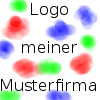
\includegraphics[height=.8\textwidth]{logo.png}
\caption{Das Logo der Musterfirma\footnotemark}
\end{figure}



%\begin{wrapfigure}{r}{.4\textwidth}
%\centering
%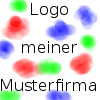
\includegraphics[height=.35\textwidth]{logo.png}
%\vspace{-15pt}
%\caption{Das Logo der Musterfirma\footnotemark}
%\end{wrapfigure}
%Quelle muss in Fußnote stehen (da sonst aufgrund eines Fehlers nicht kompiliert
% wird)
\footnotetext{aus \cite{mustermann:2012}}
Looking for the one superhero comic you just have to read. Following the antics and adventures of May Mayday Parker, this Spider-book has everything you could want in a comic--action, laughs, mystery and someone in a Spidey suit. Collects Alias \#1-28, What If. Jessica Jones had Joined the Avengers. In her inaugural arc, Jessicas life immediately becomes expendable when she uncovers the potentially explosive secret of one heros true identity. In her inaugural arc, Jessicas life immediately becomes expendable when she uncovers the potentially explosive secret of one heros true identity.

Manchmal braucht man auch Formeln. LaTeX hat einen sehr guten Formeleditor, der eigentlich selbsterklärend ist. Die Formeln weden automatisch nummeriert, aber man kann immer im Text mit einem Label wie Formel \ref{xyz} Bezug nehmen.

\begin{equation}
t-t_{0}=\sqrt{\frac{l}{g}}\int_{0}^{\varphi}{\frac{d\psi}{\sqrt{1-k^{2}\sin^{2} {\psi}}}} = \sqrt{\frac{l}{g}} F(k,\varphi)
\label{xyz}
\end{equation}

Manchmal braucht man Aufzählungen, die man in einzelnenen Punkten aufführt.
\begin{itemize}
\item Dies ist der erste Punkt, der aufgeführt wird.
\item Dies ist der zweite Punkt, der aufgeführt wird. Manchmal will man auch etwas \textbf{fett} oder \textit{kursiv} oder \textbf{\textit{beides in Kombination}}  drucken.
\item Dies ist der dritte Punkt, der aufgeführt wird.
\end{itemize}

Once upon a time, Jessica Jones was a costumed super-hero, just not a very good one. First, a story where Wolverine and Hulk come together, and then Captain America and Cable meet up. In a city of Marvels, Jessica Jones never found her niche. The classic adventures of Spider-Man from the early days up until the 90s. Looking for the one superhero comic you just have to read. In her inaugural arc, Jessicas life immediately becomes expendable when she uncovers the potentially explosive secret of one heros true identity.

Erste Erwähnung eines Akronyms wird als Fußnote angezeigt. Jede weitere wird
nur verlinkt: \gls{AGPL}. \cite{fsf:2007}

Verweise auf das Glossar: \gls{Glossareintrag}, \glspl{Glossareintrag}


%!TEX root = ../../main.tex

\chapter{Beispiel Code-schnipsel einbinden}

%title wird unter dem Bsp. abgedruckt
%caption wird im Verzeichnis abgedruckt
%label wird zum referenzieren benutzt, muss einzigartig sein.

\begin{lstlisting}[caption=Code-Beispiel, label=Bsp.1]
public class HelloWorld {
	public static void main (String[] args) {
		// Ausgabe Hello World!
		System.out.println("Hello World!");
	}
}
\end{lstlisting}

%language ändert die Sprache. (Wenn nur eine Sprache verwendet wird, kann diese Sprache in einstellungen.tex geändert werden. Standardmäßig Java.)
\begin{lstlisting}[caption=Python-Code, label=Python-Code, title=Titel des Python-Codes,language=Python]
def quicksort(liste):
if len(liste) <= 1:
	return liste
pivotelement = liste.pop()
links = [element for element in liste if element < pivotelement]
rechts = [element for element in liste if element >= pivotelement]
return quicksort(links) + [pivotelement] + quicksort(rechts)
# Quelle: http://de.wikipedia.org/wiki/Python_(Programmiersprache)
\end{lstlisting}

\section{lorem ipsum}
Looking for the one superhero comic you just have to read. Following the antics and adventures of May Mayday Parker, this Spider-book has everything you could want in a comic--action, laughs, mystery and someone in a Spidey suit. Collects Alias \#1-28, What If. Jessica Jones had Joined the Avengers. In her inaugural arc, Jessicas life immediately becomes expendable when she uncovers the potentially explosive secret of one heros true identity. 

Manchmal braucht man auch Tabellen. Ein Beispiel sieht man in Tabelle \ref{tabelle1}, welche mit einem beliebigen Label bezeichnet werden kann. Die Tabelle taucht dann automatisch im Tabellenverzeichnis auf.

\begin{table}[htb!]
\centering
\begin{tabular}{ | m{5cm} | m{1cm}| m{1cm} | } 
\hline
cell1 dummy text dummy text dummy text& cell2 & cell3 \\ 
\hline
cell1 dummy text dummy text dummy text & cell5 & cell6 \\ 
\hline
cell7 & cell8 & cell9 \\ 
\hline
\end{tabular}
\caption{Test der Funktion der Tabelle und ihrer Darstellung}
\label{tabelle1}
\end{table}


Once upon a time, Jessica Jones was a costumed super-hero, just not a very good one. First, a story where Wolverine and Hulk come together, and then Captain America and Cable meet up. In a city of Marvels, Jessica Jones never found her niche. The classic adventures of Spider-Man from the early days up until the 90s. Looking for the one superhero comic you just have to read.

Meet all of Spideys deadly enemies, from the Green Goblin and Doctor Octopus to Venom and Carnage, plus see Peter Parker fall in love, face tragedy and triumph, and learn that with great power comes great responsibility. In a city of Marvels, Jessica Jones never found her niche. Bitten by a radioactive spider, high school student Peter Parker gained the speed, strength and powers of a spider. Looking for the one superhero comic you just have to read. What do you get when you ask the question, What if Spider-Man had a daughter.

The classic adventures of Spider-Man from the early days up until the 90s. Amazing Spider-Man is the cornerstone of the Marvel Universe. But will each partner's combined strength be enough. Adopting the name Spider-Man, Peter hoped to start a career using his new abilities. Youve found it.

\section{Verweis auf Code}
Verweis auf den Code \autoref{Bsp.1}.\\
und der Python-Code \autoref{Python-Code}.

Zweite Erwähnung einer Abkürzung \gls{AGPL} (Erlärung wird nicht mehr angezeigt)

%!TEX root = ../../main.tex

\chapter{Das dritte Kapitel}
Dies ist der Text des ersten Kapitels.Nur erwähnte Literaturverweise werden auch im Literaturverzeichnis gedruckt: \cite[S.12 ff]{baumgartner:2002}, \cite[S.1-3]{dreyfus:1980}

Meine erste Fußnote\footnote{Ich bin eine Fußnote} darf auch nicht fehlen. Fußnoten sind dazu da, dass man Begriffe näher erklärt, die aber dem vertrauten Leser wahrscheinlich eh bekannt sind. 

\begin{figure}[h]
\centering
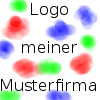
\includegraphics[height=.8\textwidth]{logo.png}
\caption{Das Logo der Musterfirma\footnotemark}
\end{figure}



%\begin{wrapfigure}{r}{.4\textwidth}
%\centering
%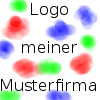
\includegraphics[height=.35\textwidth]{logo.png}
%\vspace{-15pt}
%\caption{Das Logo der Musterfirma\footnotemark}
%\end{wrapfigure}
%Quelle muss in Fußnote stehen (da sonst aufgrund eines Fehlers nicht kompiliert
% wird)
\footnotetext{aus \cite{mustermann:2012}}
Looking for the one superhero comic you just have to read. Following the antics and adventures of May Mayday Parker, this Spider-book has everything you could want in a comic--action, laughs, mystery and someone in a Spidey suit. Collects Alias \#1-28, What If. Jessica Jones had Joined the Avengers. In her inaugural arc, Jessicas life immediately becomes expendable when she uncovers the potentially explosive secret of one heros true identity. In her inaugural arc, Jessicas life immediately becomes expendable when she uncovers the potentially explosive secret of one heros true identity.

Manchmal braucht man auch Formeln. LaTeX hat einen sehr guten Formeleditor, der eigentlich selbsterklärend ist. Die Formeln weden automatisch nummeriert, aber man kann immer im Text mit einem Label wie Formel \ref{xyz} Bezug nehmen.

\begin{equation}
t-t_{0}=\sqrt{\frac{l}{g}}\int_{0}^{\varphi}{\frac{d\psi}{\sqrt{1-k^{2}\sin^{2} {\psi}}}} = \sqrt{\frac{l}{g}} F(k,\varphi)
\label{xyz}
\end{equation}

Manchmal braucht man Aufzählungen, die man in einzelnenen Punkten aufführt.
\begin{itemize}
\item Dies ist der erste Punkt, der aufgeführt wird.
\item Dies ist der zweite Punkt, der aufgeführt wird. Manchmal will man auch etwas \textbf{fett} oder \textit{kursiv} oder \textbf{\textit{beides in Kombination}}  drucken.
\item Dies ist der dritte Punkt, der aufgeführt wird.
\end{itemize}

Once upon a time, Jessica Jones was a costumed super-hero, just not a very good one. First, a story where Wolverine and Hulk come together, and then Captain America and Cable meet up. In a city of Marvels, Jessica Jones never found her niche. The classic adventures of Spider-Man from the early days up until the 90s. Looking for the one superhero comic you just have to read. In her inaugural arc, Jessicas life immediately becomes expendable when she uncovers the potentially explosive secret of one heros true identity.

Erste Erwähnung eines Akronyms wird als Fußnote angezeigt. Jede weitere wird
nur verlinkt: \gls{AGPL}. \cite{fsf:2007}

Verweise auf das Glossar: \gls{Glossareintrag}, \glspl{Glossareintrag}



\clearpage

% Bibilography

\cleardoublepage
\begin{spacing}{1.175}
    \printbibliography
\end{spacing}

% Glossar
% \cleardoublepage
% \printglossary[style=altlist,title=\glossaryPhrase]
% %!TEX root = ../main.tex

%
% To create glossary run the following command: 
% makeglossaries main.acn && makeglossaries main.glo
%

%
% Glossareintraege --> referenz, name, beschreibung
% Aufruf mit \gls{...}

\newglossaryentry{Glossareintrag}{name={Glossareintrag},plural={Glossareinträge},description={Ein Glossar beschreibt verschiedenste Dinge in kurzen Worten}}

% Abkürzungen

\newacronym{AGPL}{AGPL}{Affero GNU General Public License}


% Appendix
\clearpage

\begin{appendices}
    % \chapter{Test}


    \appendixtoc
    % \addtocontents{toc}{\protect\setcounter{tocdepth}{0}}
    % !TeX root =../main.tex

\chapter{erster Anhang}

\chapter{zweiter Anhang}

    % \addtocontents{toc}{\protect\setcounter{tocdepth}{1}}
\end{appendices}
\end{document}
